\subsubsection{\stid{3.12} Sub-project: SUNDIALS} 
\label{subsubsect:SUNDIALS-hypre}

\paragraph{Overview} 

This project is enhancing the SUNDIALS library of numerical software packages for integrating differential systems in time using state-of-the-art time step technologies for use on exascale systems.  

The SUNDIALS suite of packages provides efficient and adaptive time integrators and nonlinear solvers.  The packages are written using encapsulation of both data structures and solvers, thus allowing easy incorporation into existing codes and flexibility to take advantage of new solver technologies and packages.  SUNDIALS provides both multistep and multistage methods designed to evolve stiff or nonstiff ordinary (ODE) and differential algebraic (DAE) systems
with efficient accuracy-driven time step selection.
SUNDIALS also provides both Newton and fixed point (with optional acceleration) nonlinear solvers and scaled Krylov methods with hooks for user-supplied preconditioners.  Users can also supply their own nonlinear and linear solvers under the integrators.  SUNDIALS is released with data structures supporting several programming environments.  Users can employ these supplied structures or provide their own. 

Through software infrastructure developments, this project is enabling the efficient and robust SUNDIALS time integrator packages to easily interoperate with applications evolving time dependent systems as well as with external linear and nonlinear solver packages developed for exascale computing.  In addition, this project is providing support for integrating several independent ordinary differential equation systems simultaneously on GPUs as part of multiphysics applications.  Lastly, this project is supporting the deployment and use of SUNDIALS packages within ECP applications, mainly through incorporation into the discretization-based Co-Design Centers, AMReX and CEED.

%% Efficient time integrators are essential for ECP because they are at the core of every time-dependent simulation application.  However, many applications do not use state-of-the-art methods, and if they do, they often do not yet use them fully on their systems.  For example, at the start of the ECP the astrophysics code, Nyx, used an adaptive integration package for solving individual reactions.  However, by applying a time integration package to a larger reaction system, the code is able to derive significant speedups through use of GPUs that execute more calculations concurrently thus getting an accurate solution much faster.  By allowing for solvers tuned to exascale systems and vectors that are heterogeneous, SUNDIALS will be more applicable for use in multiphysics systems running on exascale platforms.


\paragraph{Key Challenges}

Current implementations of efficient time integrators face challenges on many fronts.  
First, applications need both efficient integrators and ones that can interface easily with efficient linear algebra
packages to solve subservient linear systems.  In addition, integrators and their interfaces to both solver libraries 
and applications must be frequently updated to keep up with rapid advances in system architectures. Some ECP applications require solution of many small systems of ODEs in parallel on GPUs giving rise to the need for 
a GPU-enabled ODE integrator that can be used in parallel for many systems at once. Lastly, ECP applications are in need of ODE integrators that can provide increasing functionalities, such as non-identity mass matrices for solving systems of ODEs with finite element spatial discretizations, and maintaining solutions on a constraint manifold.

\paragraph{Solution Strategy}

This project includes a number of implementation activities that will prepare the SUNDIALS suite of time integrators for exascale systems found in ECP applications.  A major activity is the development of support for using the CVODE multistep
ODE integration package to evolve multiple systems of ODEs in parallel using GPUs.  Two strategies are being pursued for this capability.  First, multiple ODE systems are being integrated in each CVODE instance with multiple instances started on a GPU, each with a different CUDA stream.  In this case, CVODE is being equipped with a batched direct linear 
solver capable of using a GPU.  In addition, differing methods of choosing time steps and nonlinear solver convergence strategies are being investigated to help optimize performance of CVODE on these aggregated systems.  The second strategy is development of a version of CVODE callable on a GPU, although this strategy is most appropriate for very small ODE systems.  

This project is also developing efficient ways of handling time-dependent mass matrices for use by the ARKode multistage integrator package and use from within the MFEM library.  This capability will likely be supported at the system function evaluation level and will make finite element methods much more efficient with the 
SUNDIALS multistage integrator.  In order to handle ODE systems with constraint manfiolds, an older package, CPODES, is being evaluated and rewritten with the current SUNDIALS interfaces.  This constraint manifold capability will be interfaced with ECP application codes for method evaluation and testing.  

Lastly, the SUNDIALS team will support ECP applications in interfacing SUNDIALS packages into their
software and in the optimal use of the time integration algorithms.  This support will also include working with the application teams to help them install SUNDIALS and adjust their build systems to appropriately link with the SUNDIALS library. 

%%  A major activity is a redesign of all linear solver interfaces and encapsulation of the nonlinear solvers within the time integrators in SUNDIALS.  The new linear solver interfaces make it much easier to interface external solver packages while maintaining the efficiency of SUNDIALS integrators. Encapsulating the nonlinear solvers reduces redundant code and allows the time integrators to better leverage common code resulting in a lower code maintenance burden within SUNDIALS.  In addition, the integrators are able to take advantage of outside nonlinear solvers.  

%% This project also introduced a set of optional fused vector kernels into SUNDIALS.  These kernels execute multiple vector operations at once thereby reducing the number of kernel launches in GPU environments and also reducing the number of communications required for reduction operations.  These new kernels were added to all supplied SUNDIALS vectors and are invoked through optional interfaces.

%% Lastly, this project is developing a many-vector capability for SUNDIALS.  Due to the tight data encapsulation within SUNDIALS, users are able to supply any vector they would like underneath the integrators.  This project will supply the infrastructure needed to make it easy to place a vector of vectors underneath the integrators.  This vector of vectors is essential for later implementation of time integrators that will advance various parts of the system with different time step sizes.  This many-vector capability will also ease the use of different programming environments as differing vectors can be instantiated on different parts of a hybrid machine. 

\paragraph{Recent Progress}

In October of 2019, SUNDIALS 5.0.0 was released, including new vector structures that support flexible partitioning of solution data among different processing elements (e.g., CPU + GPU) or for multi-physics problems, an additional vector structure that supports MPI+X paradigms, and interfaces 
to high performance algebraic solver packages (SUPERLU\_DIST, the NVIDIA CUDA-based 
batched sparse QR direct linear solver, and the PETSc nonlinear solver SNES package).
In September of 2019, the SUNDIALS team released a document quantifying performance of SUNDIALS codes on 
a demonstration problem that solves the three-dimensional nonlinear compressible Euler equations combined with advection and reaction of chemical species run using 40 cores on each of 2 to 3,456 nodes of the ORNL Summit machine.
Figure \ref{fig:sun-many-demo} shows a diagram of the many-vector used in the demonstration problem where some solution components are distributed across the MPI processor decomposition and some are fully local.
In addition to these activities, the SUNDIALS team has been collaborating closely with the AMReX Co-Design Center team to 
design effective interfaces to SUNDIALS time integrators from AMReX for applications using ODE integrators,
such as for chemistry reaction systems as in Nyx, Castro, and PELE.  The PELELM and Nyx applications have both demonstrated use of the CVODE package from SUNDIALS within test runs utilizing new capabilities from SUNDIALS to run on Summit with GPUs.


%% In May of 2018, SUNDIALS 4.0.0-dev was released, including new fused vector kernels in the vector API and in all supplied vectors.  Results show speedup from using these routines, especially for parallel reductions.  In September of 2018, SUNDIALS 4.0.0-dev.2 was released, including a full redesign of the nonlinear solver interfaces to the time integrators and encapsulation of the nonlinear solevrs.  Figure \ref{fig:sunorg1} shows the new organization of SUNDIALS where separate nonlinear solver interfaces are provided for Newton and fixed point nonlinear solver methods.  These interfaces are shared across all SUNDIALS integrators.  
%% Individual integrators have the freedom to supply specific information from the integrator that controls the solver.  In addition, the SUNDIALS team has been collaborating closely with the AMReX Co-Design Center team to 
%% design effective interfaces to SUNDIALS time integrators from AMReX for applications using ODE integrators,
%% such as for chemistry reaction systems as in Nyx, Castro, and PELE.

\begin{figure}[htb]
	\centering
	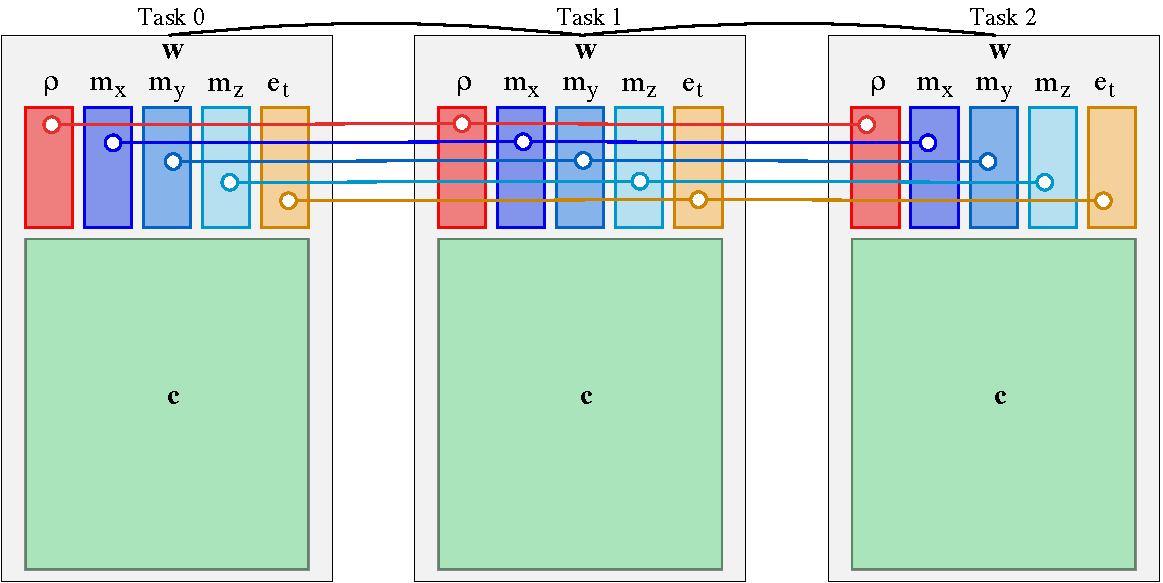
\includegraphics[width=6in]{projects/2.3.3-MathLibs/2.3.3.12-SUNDIALS-hypre/manyvector_v2.pdf}
	\caption{\label{fig:sun-many-demo}The demonstration code uses the new many-vector capability to store the solution as a collection of distributed ($\rho,m_i, e_t$) and purely local ($c$) vectors.}
\end{figure}




\paragraph{Next Steps}

During the remainder of FY20, this project team will:
\begin{enumerate}
\item Release SUNDIALS with new CVODE options for solving multiple ODE systems in parallel on GPUs.
\item Complete a prototype of CPODES.
\item Release of SUNDIALS with a time-dependent mass matrix capability.
\item Continue to support AMReX and CEED Co-Design Centers in their use of SUNDIALS for ECP applications.
\end{enumerate}
